%%%%%%%%%% *** The Title %%%%%%%%%%
\title[]{대기오염\\\small{제13장}}

\begin{frame}[plain] %title page
	\titlepage
\end{frame}


\section{대기오염의 위협}


\begin{frame}[t]{대기 오염의 정의}
	\begin{tabular}{ll}
		\begin{minipage}[t]{0.94\textwidth}\scriptsize
			\begin{itemize}
				\item 대기 중에 인위적으로 배출된 오염물질이 한 가지 또는 그 이상이 존재하여, 오염물질의 양과 농도 및 지속시간에 따라 어떤 지역의 불특정 다수에게 불쾌감을 일으키거나 해당지역에 공중보건상의 위해를 끼치고, 인간이나 동식물의 활동에 위해를 주어 생활과 재산을 향유할 정당한 권리를 방해받는 상태(세계보건 기구, WHO)
				\item 대기 오염은 외기 중에 1종 이상의 오염 물질이 존재하여, 이러한 물질의 성질과 존속에 의해 인체, 동식물 및 재산에 피해를 주거나, 혹은 쾌적한 생활 및 재산에 부당하게 관여되는 것(미국 기술자 총연합회)
				\item 사람, 동식물의 생명 혹은 재산에 해가 되거나 해가 될 정도로 충분한 양만큼, 그리고 충분한 기간 동안 1가지 혹은 그 이상의 오염물질이 대기에 존재하는 것(애리조나주 대기 오염 규정)
				\item 대기 오염이란 대기의 자정 능력 이상의 오염물질이 대기 중에 방출되어 특정 지역의 다수인에게 불쾌감을 주는, 혹은 인간과 동식물 및 재산에 유해하고 쾌적한 생활을 방해하는 대기 상태(대기과학개론)
			\end{itemize}

		\end{minipage}	
		&
		\begin{minipage}[t]{0.01\textwidth} \scriptsize	
			
		\end{minipage}
	\end{tabular}
\end{frame}



\begin{frame}[t]{대기오염의 역사}
	\begin{tabular}{ll}
		\begin{minipage}[t]{0.94\textwidth}\scriptsize
			
			대기 오염은 20 세기에 들어서 갑자기 나타난 것이 아니라 대략 11세기부터 서서히 발생해 왔음.
			\begin{itemize}
				\item 석탄 연소 금지 선언(1300년 경, 영국 에드워드 1세)
				\item 석탄 사용 금지(1578년, 엘리자베드 1세)
				\item 런던 도시 공장 이전 및 녹지대 설정(1661년, 에브린)
				\item 대기 오염 연구 위한 선발위원회 구성(1741, 1843, 1845)
				\item 가축의 참사 사건(1875년)
				\item 벨기에 뮤즈(Meuse) 계곡(1930), 일본 도쿄-요코하마 천식(1946), 미국 도노라(1948) 사건
				\item 런던 스모그(1952), 로스앤젤레스 스모그(1954) 사건
				\item 우리나라는 1960년대 말부터 대기 오염이 나타났으며, 1970년대부터 심화됨
				\item 대규모 사망 사건은 없었으나 대기 오염에 의한 분쟁 건수가 증가 추세
				
			\end{itemize}

		\end{minipage}	
		&
		\begin{minipage}[t]{0.01\textwidth} \scriptsize	
			
		\end{minipage}
	\end{tabular}
\end{frame}



\begin{frame}[t]{오염물질 발생원}
	\begin{tabular}{ll}
		\begin{minipage}[t]{0.55\textwidth}\scriptsize
			\begin{figure}[t]
				\includegraphics[trim=290 420 50 120, clip, 
				page=391, width=\textwidth]{\bookfile}
			\end{figure}
		\end{minipage}	
		&
		\begin{minipage}[t]{0.4\textwidth} \scriptsize	
			\begin{itemize}
				\item 인위적 발생원: 연소 과정, 화학 작용 과정, 원자력 과정, 굽기, 가열 제련과정, 채광 채석, 농업 등
				\item 자연적 발생원원: 화산, 부서지는 파도, 꽃가루, 테르펜, 화재, 날리는 먼지, 세균, 바이러스 등
			\end{itemize}

		\end{minipage}
	\end{tabular}
\end{frame}



\begin{frame}[t]{자연적 발생원}
	\begin{tabular}{ll}
		\begin{minipage}[t]{0.55\textwidth}\scriptsize
			\begin{figure}[t]
				\includegraphics[trim=45 50 350 470, clip, 
				page=391, width=\textwidth]{\bookfile}
			\end{figure}
		\end{minipage}	
		&
		\begin{minipage}[t]{0.4\textwidth} \scriptsize	
			인간 활동과 관계없이 오염 물질을 발생시키는 발생원으로 농도가 높지는 않지만, 주변에 항시 존재
			\begin{itemize}
				\item 화산폭발: 화산재, 가스(황 산화물, 메탄) 방출
				\item 산불: 매연, 탄화 수소, CO, 질소 산화물 방출
				\item 해양: 해염입자
			\end{itemize}

		\end{minipage}
	\end{tabular}
\end{frame}



\begin{frame}[t]{인위적 발생원}
	\begin{tabular}{ll}
		\begin{minipage}[t]{0.5\textwidth}\scriptsize
			\begin{figure}[t]
				\includegraphics[trim=350 0 0 520, clip, 
				page=392, width=\textwidth]{\bookfile}
			\end{figure}
		\end{minipage}	
		&
		\begin{minipage}[t]{0.45\textwidth} \scriptsize	
			인간 활동에 기인한 것 발생원
			\begin{itemize}
				\item 가정 난방이나 발전소의 원료(목재, 석탄, 석유)에 의해 아황산 가스, 질소 산화물
				\item 공장의 중금속 등 오염물질 배출
			\end{itemize}

		\end{minipage}
	\end{tabular}
\end{frame}


\begin{frame}[t]{인간 활동에 기인한 자연적 대기오염}
	\begin{tabular}{ll}
		\begin{minipage}[t]{0.55\textwidth}\scriptsize
			\begin{figure}[t]
				\includegraphics[trim=0 440 200 0, clip, 
				page=392, width=\textwidth]{\bookfile}
			\end{figure}
		\end{minipage}	
		&
		\begin{minipage}[t]{0.4\textwidth} \scriptsize	
			\begin{itemize}
				\item 농지 개간으로 인해 식생이 사라져서 발생한 대기오염 사례 
			\end{itemize}

		\end{minipage}
	\end{tabular}
\end{frame}



\section{대기오염의 근원과 형태}

\begin{frame}[t]{대기 오염물질의 분류}
	\begin{tabular}{ll}
		\begin{minipage}[t]{0.55\textwidth}\scriptsize
			\begin{figure}[t]
				\includegraphics[trim=40 40 350 550, clip, 
				page=393, width=\textwidth]{\bookfile}
			\end{figure}
		\end{minipage}	
		&
		\begin{minipage}[t]{0.4\textwidth} \scriptsize	
			
			대기 오염원은 생물체의 건강과 복지를 위협할 수 있는 농도를 가진 입자와 가스
			\begin{itemize}
			\item 입자상 오염물질(분진, 에어로졸): 먼지, 스모그, 안개 등 포함한 고체와 액체
			\item 가스(기체)상 물질: 탄소 산화물, 황 산화물, 질소 산화물 등
			\end{itemize}					
			
		\end{minipage}
	\end{tabular}
\end{frame}




\begin{frame}[t]{1차/2차 오염 물질}
	\begin{tabular}{ll}
		\begin{minipage}[t]{0.55\textwidth}\scriptsize
			\begin{figure}[t]
				\includegraphics[trim=40 40 350 550, clip, 
				page=393, width=\textwidth]{\bookfile}
			\end{figure}
		\end{minipage}	
		&
		\begin{minipage}[t]{0.4\textwidth} \scriptsize	
			
			\begin{itemize}
				\item 1차 오염물질: 오염원에서 직접 대기로 방출되어 방출 즉시 대기를 오염시킴
				\item 2차 오염물질: 1차 오염원들의 화학반응에 의해 대기 중에서 생성
				
				오존, 질소 산화물, 휘발성 유기물질이 강한 태양 빛을 매개로 다량의 유독성을 지닌 2차 오염물을 생성함. 
			\end{itemize}

		\end{minipage}
	\end{tabular}
\end{frame}




\begin{frame}[t]{입자상 물질(Particulate Matter: PM)}
	\begin{tabular}{ll}
		\begin{minipage}[t]{0.4\textwidth}\scriptsize
			\begin{figure}[t]
				\includegraphics[trim=330 410 50 100, clip, 
				page=393, width=\textwidth]{\bookfile}
			\end{figure}
		\end{minipage}	
		&
		\begin{minipage}[t]{0.55\textwidth} \scriptsize	
			가벼운 것은 대기 중에서 떠다님, 가스상 오염물질보다는 극히 적은 양이지만, 큰 영향을 미침

			총 부유 분진(TSP): 지름 45 $\rm{\mu m}$ 이하인 모든 입자의 총량

			미세먼지($\rm{{PM}_{10}}$): 지름이 10 $\rm{\mu m}$ 이하인 입자로 보통 비포장 도로의 운송, 분쇄, 압착 등의 과정에서 발생

			초미세먼지($\rm{{PM}_{2.5}}$): 지름이 2.5 $\rm{\mu m}$ 이하인 입자로 교통 수단, 발전소, 공장의 연료 소비와 주택 난방에 의해 발생
	
		\begin{itemize}
				\item 생물분진 : 진드기, 박테리아와 바이러스, 꽃가루 등
				\item 자동차 매연, 공장의 굴뚝 연기, 제철소나 소각장 등의 먼지, 쓰레기 불법 연소
				\item 사람이 움직일 때, 요리할 때 등
				\item 해염(파도가 부서질 때 생기는 소금 알갱이)
				\item 황사, 화산재나 유성의 재
									
			\end{itemize}

		\end{minipage}
	\end{tabular}
\end{frame}



\begin{frame}[t]{입자상 물질의 영향}
	\begin{tabular}{ll}
		\begin{minipage}[t]{0.5\textwidth}\scriptsize
			인체에 미치는 영향
			\begin{itemize}	
				\item 0.5 $\rm{\mu m}$ 보다 큰 입자들은 코와 목에서 주로 침적되며, 기관지나 기도를 잘 통과하지 못하고 코와 목의 섬모운동에 의해 곧 제거됨.
				\item 0.5 $\rm{\mu m}$ 보다 작은 입자들은 폐포까지 도달하여 침적될 수 있으며, 이 입자들은 제거가 서서히 진행되고 완전한 제거는 불가능. 이러한 입자의 일부는 혈관으로 흡수되기도 함.
				\item 분진 자체의 독성이 영향을 주거나 다른 유해물질의 제거에 방해를 하는 역할
				\item $\rm{{PM}_{10}}$은 천식과 같은 호흡기 질환을 악화시킴
				\item $\rm{{PM}_{2.5}}$는 급성 호흡기 질환, 폐 기능 저하, 신생아 사망과 관련
				\item 진폐증, 폐선유증, 폐기종 등은 미세분진의 축적으로 인한 증상
			\end{itemize}
			
		\end{minipage}	
		&
		\begin{minipage}[t]{0.45\textwidth}
			\begin{figure}[t]
				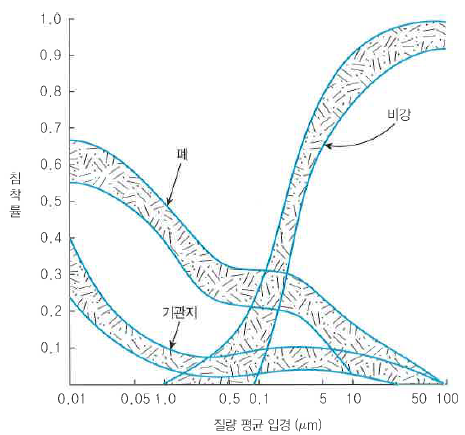
\includegraphics[width=\linewidth]{images/tsp.png}
			\end{figure}
			
		\end{minipage}
	\end{tabular}
\end{frame}



\begin{frame}[t]{입자상 물질의 영향}
	\begin{tabular}{ll}
		\begin{minipage}[t]{0.475\textwidth}\scriptsize
			\begin{itemize}			
				\item 식물에 미치는 영향: 시멘트 먼지는 미스트나 작은 빗방울과 결합할 때, 잎의 표면에 두꺼운 막을 형성하여 태양광을 차단하고 광합성을 저해하여 식물의 성장을 막음							
				\item 분진은 대개 점성이 있고 산성을 띠고 있어서 표면에 부착되면 페이팅이나 건축 현장에 피해를 줌.
				\item 태양빛을 산란하여 시정을 감소시킴 ($0.1 \sim 1.0 \rm {\mu m}$ 일 때 산란도 최대)
				\item 분진의 산란과 흡수에 의해 지표면에 도달하는 태양복사량 감소시킴
				\item 수분을 응축할 수 있는 핵과 같은 역할을 하므로, 대기 중의 분진의 양이 증가하면 강수량이 증가될 수 있음.
			\end{itemize}

		\end{minipage}	
		&
		\begin{minipage}[t]{0.475\textwidth} \scriptsize	
			
		\end{minipage}
	\end{tabular}
\end{frame}



\begin{frame}[t]{가스상 물질: 이산화 황($\rm{{SO}_{2}}$)}
	\begin{tabular}{ll}
		\begin{minipage}[t]{0.475\textwidth}\scriptsize
			\begin{itemize}
				\item 석탄이나 석유와 같이 황을 포함한 연료가 연소될 때 방출되는 무색 기체
				\item 주요 방출원: 발전소, 제련소, 제지공장, 정유시설
				\item 이산화 황과 산소 분자와의 반응으로 삼산화 황이 생성되고, 물 분자와의 빠른 반응에 의해 황산이 생성됨. 이렇게 생성된 황산은 황산 미스트 혹은 황산 에어로졸임.
			\end{itemize}
		\end{minipage}	
		&
		\begin{minipage}[t]{0.475\textwidth} \scriptsize	
			\begin{itemize}
				\item 황산 에어로졸은 폐포를 자극하여 팽창시키며, 그 결과 작은 폐포가 엉겨 붙어 큰 폐포가 되면서 산소와 이산화 탄소를 교환하는 호흡 면적을 감소시켜, 호흡 곤란 증세를 유발함.
				\item 특정한 사람(노약자, 심장 혹은 호흡 기계통의 만성 질환자)에게 심각한 영향을 줌
				\item 천식 증상을 지닌 아이나 야외 활동하는 성인들의 호흡기 질환 및 폐기능 약화, 장기간 노출시 심장 질환 유발
				\item 저농도에서도 호흡기 자극, 용해도가 높아 기도에 용이하게 흡수, 기관지 점막 자극하여 가래 유발
				\item 산성비의 원인(부식성): 대기 중 황산입자가 비와 눈과 함께 풍하측에서 하강
			\end{itemize}
		\end{minipage}
	\end{tabular}
\end{frame}




\begin{frame}[t]{가스상 물질: 질소 산화물($\rm{{NO}_{x}}$)}
	\begin{tabular}{ll}
		\begin{minipage}[t]{0.475\textwidth}\scriptsize
			\begin{itemize}
				\item 질소 성분이 포함된 연료를 고온으로 연소시킬 때 산소와 결합하여 생성
				\item 세균에 의한 생분해 과정에서 생성되기도 함
				\item 도시 내의 질소 산화물 농도가 교외 지역보다 $10 \sim 100$ 배 더 높음 
				(즉, 자연적으로 생성되는 경우보다 인간 활동에 의한 요소가 큼)
				\item 주요 방출원: 자동차, 발전소(엔진의 연소)
				\item 일산화질소($\rm{NO}$)가 대기 중에 방출되어 시간이 경과되면 이산화질소($\rm{{NO}_{2}}$)로 변화
				\item 질소 산화물은 일산화질소와 이산화질소를 통칭한 의미
				\item 붉은 갈색, 악취를 가진 자극성 가스로 반응성이 커 스모그 형성
			\end{itemize}
		\end{minipage}	
		&
		\begin{minipage}[t]{0.475\textwidth} \scriptsize	
			\begin{itemize}
				\item 급성 피해(고농도 단기간 노출): 눈과 코를 강하게 자극하고, 폐출혈 및 폐수종, 폐색성 기관지염을 일으켜 사망에 이르게 함.
				\item 만성 피해(저농도 장기간 노출): 만성 폐섬유화, 폐수종 유발
				\item 식물의 잎에 반점 생성, 광합성 속도 저하, 잎의 색 변화
				\item 산성비의 원인: 이산화질소는 수증기와 반응하여 질산($\rm{{HNO}_{3}}$)을 생성하며, 부식성을 가진 산성비의 원인이 되기도 함
			\end{itemize}
		\end{minipage}
	\end{tabular}
\end{frame}




\begin{frame}[t]{가스상 물질: 일산화 탄소($\rm{{CO}}$)}
	\begin{tabular}{ll}
		\begin{minipage}[t]{0.475\textwidth}\scriptsize
			$$
				\mathrm{C}+\frac{1}{2} \mathrm{O}_{2} \longrightarrow \mathrm{CO}+29,400 \mathrm{kcal} / \mathrm{kmol}
			$$
			\begin{itemize}
				\item 석탄, 나무, 석유 등의 불완전 연소시 발생하는 무색, 무취의 유독성 기체
				\item 주요 방출원 : 자동차, 폐기물 소각, 제철소, 가정용 난방 등 연소시설의 불완전 연소
				\item 가정용 난방 및 취사 연료가 석유와 도시가스로 전환되면서 자동차가 주된 방출원이 됨
				\item 박테리아의 활동에 의해 이산화탄소로 산화되어 대기에서 제거, 대류권과 성층권에서 광화학 반응에 의해서 제거되기도 함
				\item 반응성이 매우 높아 스모그 형성에 중요한 역할
				\item 붉은 갈색을 띄며, 시정을 감소시킴
			\end{itemize}

		\end{minipage}	
		&
		\begin{minipage}[t]{0.475\textwidth} \scriptsize	
			
			$$
				\mathrm{CO}+\mathrm{OH} \stackrel{\mathrm{O}_{2}}{\longrightarrow} \mathrm{CO}_{2}+\mathrm{HO}_{2} 
			$$
			$$
				\mathrm{CO}+\mathrm{OH} \longrightarrow \mathrm{CO}_{2}+\mathrm{H}
			$$
				
			위의 과정으로 대기 중에서 빠르게 제거되지만, 물에 난용성이기 때문에 강수에 영향을 받지 않으며, 다른 오염물질과 반응하지 않고 흡착되지도 않아 체류기간이 짧지 않음
			
		\end{minipage}
	\end{tabular}
\end{frame}



\begin{frame}[t]{$\rm{{CO}}$ 배출}
	\begin{tabular}{ll}
		\begin{minipage}[t]{0.5\textwidth}\scriptsize
			\begin{figure}[t]
				\includegraphics[trim=350 50 50 450, clip, 
				page=396, width=\textwidth]{\bookfile}
			\end{figure}
		\end{minipage}	
		&
		\begin{minipage}[t]{0.45\textwidth} \scriptsize	
			\begin{itemize}
				\item 아마존과 동남아시아 지역의 일산화탄소 고농도는 화재가 주요 배출원
				\item 미국, 유럽, 중국은 자동차와 공장이 주요 배출원
			\end{itemize}
		\end{minipage}
	\end{tabular}
\end{frame}




\begin{frame}[t]{산불과 대기 오염}
	\begin{tabular}{ll}
		\begin{minipage}[t]{0.4\textwidth}\scriptsize
			\begin{figure}[t]
				\includegraphics[trim=40 260 350 170, clip, 
				page=395, width=\textwidth]{\bookfile}
			\end{figure}
		\end{minipage}	
		&
		\begin{minipage}[t]{0.55\textwidth} \scriptsize	
			\questionset{산불은 적란운 발달에 어떻게 영향을 미치는가?}
			\solutionset{산불로 인해 데워진 공기는 강한 상승기류를 야기시켜 적란운이 발달할 수 있다. }
		\end{minipage}
	\end{tabular}
\end{frame}




\begin{frame}[t]{대기 오염과 기후}
	\begin{tabular}{ll}
		\begin{minipage}[t]{0.5\textwidth}\scriptsize
			\begin{figure}[t]
				\includegraphics[trim=350 440 30 100, clip, 
				page=394, width=\textwidth]{\bookfile}
			\end{figure}
		\end{minipage}	
		&
		\begin{minipage}[t]{0.45\textwidth} \scriptsize	
			\questionset{겨울철 고위도 지역의 도시에서 대기 오염 에피소드는 여름철 유사한 이벤트 보다 표면에 도달하는 태양에너지의 비율이감소할 가능성이 있다. 왜 그러한가?}
			\solutionset{대도시의 입자상 물질에 의해 태양 복사 에너지의 15 \% 이상 감소하고, 
					자외선은 30\% 이상 감소한다. 겨울철 고위도 지역은 태양의 고도가 낮아 햇빛이 통과하는 대기층이 길어 지표면에 도달하는 태양복사에너지가 더욱 많이 감소할 것이다. }

		\end{minipage}
	\end{tabular}
\end{frame}



\begin{frame}[t]{에너지 소비}
	\begin{tabular}{ll}
		\begin{minipage}[t]{0.65\textwidth}\scriptsize
			\begin{figure}[t]
				\includegraphics[trim=50 340 110 50, clip, 
				page=396, width=\textwidth]{\bookfile}
			\end{figure}
		\end{minipage}	
		&
		\begin{minipage}[t]{0.3\textwidth} \scriptsize	
			\begin{itemize}
				\item 완쪽은 우리가 어떤 에너지를 사용하는지, 				
				\item 오른쪽은 그 에너지가 어디에 사용되는지 예를 보여준다.
				
			\end{itemize}

		\end{minipage}
	\end{tabular}
\end{frame}


\begin{frame}[t]{휘발성 유기 화합물(VOCs)}
	\begin{tabular}{ll}
		\begin{minipage}[t]{0.475\textwidth}\scriptsize
			휘발성 유기 화합물 (Volatile Organic Compounds, VOC) 탄화 수소라고도 부르며, 고체, 액체, 기체의 형태를 모두 띨 수 있음
			\begin{itemize}
				\item 주요 방출원
				 	1) 식물에서 방출(자연적 배출원) : 기후 변화에 영향, 광화학 반응에 의한 오존 생성에 영향 
					2) 공장 도장 공정 등 유기용제 사용, 불완전 연소된 가솔린(인위적 배출원)
				\item VOCs는 자체로 큰 환경문제를 야기하거나 건강에 직접적 영향을 미치는 경우는 드물지만, 장기간 노출될 경우에는 만성적 피해를 유발할 수 있음.
				\item 질소 산화물의 광분해 반응에 관여하여 2차 오염물질 형성(오존 등)에 큰 영향
					
			\end{itemize}
		\end{minipage}	
		&
		\begin{minipage}[t]{0.475\textwidth} \scriptsize	
			

		\end{minipage}
	\end{tabular}
\end{frame}




\begin{frame}[t]{납($\rm{{Pb}}$)	}
	\begin{tabular}{ll}
		\begin{minipage}[t]{0.475\textwidth}\scriptsize
			\begin{itemize}
				\item 과거에는 엔진 노킹(knocking) 현상을 막기 위해 자동차 연료에 납을 첨가하여 주요 오염원으로 자동차가 등장했으나 최근에는 1970년대 이후 ‘무연’휘발유를 활용하면서 대기 중의 납 농도는 많이 낮아짐
				\item 노후 건물의 벗겨진 페인트 조각도 오염원
				\item 유입된 납의 일부가 혈액, 중추신경, 장기(간, 폐) 등에 축적되며 장기 손상을 일으킴.
				\item 고농도에 단기간 노출시, 지능 저하, 행동 장애, 심장 질환, 사망을 유발함. 
				\item 태아가 성숙하는 동안 해를 끼치므로, 임산부가 납에 노출되면 조산하거나 저체중 아이를  출산하거나 유산할 수 있음
			\end{itemize}
		\end{minipage}	
		&
		\begin{minipage}[t]{0.475\textwidth} \scriptsize	
			
		\end{minipage}
	\end{tabular}
\end{frame}


\begin{frame}[t]{2차 오염물질: 오존($\rm{{O}_{3}}$)}
	\begin{tabular}{ll}
		\begin{minipage}[t]{0.475\textwidth}\scriptsize
			성층권에서 자연적으로 생성되며, 인간 활동의 영향으로 지표면 부근에서도 생성된 오존은 광화학 스모그의 주요 요소임.
				NO2의 광분해 순환과정
				$$
					\begin{array}{l}
					\mathrm{NO}_{2}+h \mathrm{v} \rightarrow \mathrm{NO}+\mathrm{O} \\
					\mathrm{O}+\mathrm{O}_{2}+\mathrm{M} \rightarrow \mathrm{O}+\mathrm{M} \\
					\mathrm{O}_{3}+\mathrm{NO} \rightarrow \mathrm{NO}_{2}+\mathrm{O}_{2}
					\end{array}
				$$

			\begin{itemize}
				\item 오존의 생성 반응은 강한 일사에 의해 발생하므로 대기 중의 오존은 낮 시간에 한정되어 형성되며, 
				\item 1년 중 여름에 오존 농도가 가장 높음
			\end{itemize}

		\end{minipage}	
		&
		\begin{minipage}[t]{0.475\textwidth} \scriptsize	
			\begin{itemize}
				\item 급성적인 눈의 통증, 극심한 피로와 인체 조정 기능 손실, 폐 기능 손상 등
				\item 가슴통증, 심장질환 유발, 호흡기 질병 악화
				\item 천연 및 인조 섬유에 화학반응을 일으켜 탄소 원자의 구조가 변화됨
				\item 고무에 아주 작은 외력이 작용하면 물리적 변형 발생(타이어는 오존 산화에 매우 취약)
			\end{itemize}
		\end{minipage}
	\end{tabular}
\end{frame}



\begin{frame}[t]{스모그(Smog)}
	\begin{tabular}{ll}
		\begin{minipage}[t]{0.6\textwidth}\scriptsize
			\begin{itemize}
				\item 도시와 공장 지역에서의 대기 오염을 스모그 현상이라고 함 (연기 smoke+안개 fog)
				\item 원래 의미는 석탄 연소의 부산물과 높은 습도 상태가 결합되어 나타난 대기 오염 상태를  의미하였음
				\item 오늘날 스모그는 일반적인 대기 오염을 통칭하며, 연기와 안개의 결합을 엄격하게 적용하지는 않음.
			\end{itemize}
		\end{minipage}	
		&
		\begin{minipage}[t]{0.35\textwidth} \scriptsize	
			

		\end{minipage}
	\end{tabular}
\end{frame}



\begin{frame}[t]{런던형(고전형) 스모그}
	\begin{tabular}{lll}
		\begin{minipage}[t]{0.25\textwidth}\scriptsize
			\begin{figure}[t]
				\includegraphics[trim=320 380 80 110, clip, 
				page=397, width=\textwidth]{\bookfile}
			\end{figure}
		\end{minipage}	
		&
		\begin{minipage}[t]{0.25\textwidth}\scriptsize
			\begin{figure}[t]
				\includegraphics[trim=50 380 350 110, clip, 
				page=398, width=\textwidth]{\bookfile}
			\end{figure}
		\end{minipage}	
		&
		\begin{minipage}[t]{0.45\textwidth} \scriptsize	
			\begin{itemize}
				\item 1952년 런던에서는 고기압의 정체로 인한 안정한 대기 상태에서 복사역전층이 형성되고 무풍 상태가 지속되면서, 짙은 안개가 끼고 먼지와 아황산 가스 농도가 급격히 상승함
				심장질환자, 호흡기 환자 급증하며 사망자 속출
				\item 오염 발생원은 가정 난방용 석탄의 매연과 화력발전소에서 배출된 매연으로 추정
				\item 안개입자에 흡수된 아황산 가스가 석탄먼지의 촉매작용으로 황산미스트를 형성
				\item 1956년 청정공기법을 제정하고 특정 지역의 석탄 사용 금지
					
			\end{itemize}

		\end{minipage}
	\end{tabular}
\end{frame}






\begin{frame}[t]{광화학(LA형) 스모그}
	\begin{tabular}{ll}
		\begin{minipage}[t]{0.45\textwidth}\scriptsize
			\begin{figure}[t]
				\includegraphics[trim=0 410 340 0, clip, 
				page=404, width=\textwidth]{\bookfile}
			\end{figure}
		\end{minipage}	
		&
		\begin{minipage}[t]{0.5\textwidth} \scriptsize	
			\begin{itemize}
				\item LA는 연중 침강역전층이 형성되고 해안성 안개가 끼는 도시임.
				\item 강한 태양빛을 매개로 2차 오염물질 형성하는 반응
				\item (예시) VOCs가 강한 햇빛을 받아 광화학 반응을 하면 반응성, 자극성, 유독성을 지닌 2차 오염물질이 생성
				\item (예시) 질소 산화물이 태양빛에 의해 광화학 반응을 바면 오존을 생성함
				\item 다수의 자동차에서 배출되는 질소 산화물과 탄화 수소는 여름철 자외선에 의해 오존을 포함한 광화학 스모그 물질을 생성
				\item 즉, 1차 오염물질이 햇빛이 강한 여름철에 2차 오염물질을 생성한 것
			\end{itemize}

		\end{minipage}
	\end{tabular}
\end{frame}



\begin{frame}[t]{광화학(LA형) 스모그}
	\begin{tabular}{ll}
		\begin{minipage}[t]{0.45\textwidth}\scriptsize
			\begin{figure}[t]
				\includegraphics[trim=0 410 340 0, clip, 
				page=404, width=\textwidth]{\bookfile}
			\end{figure}
		\end{minipage}	
		&
		\begin{minipage}[t]{0.5\textwidth} \scriptsize	
			\questionset{LA에서 발생하는 대기 오염에 영향을 주는 요인을 세 가지로 설명하시오.}
			\solutionset{1)LA는 북태평양 고기압에 의한 하강 기류와 관련된 기온역전이 빈번하게 나타남.

				2)태평양으로부터 이동해 온 공기가 차가운 해류에 의해 차가워지고 LA 지역의 따뜻한 공기와 만나면서 따뜻한 공기가 상승하며 기온 역전이 나타남.

				3)주변 산들이 도시 스모그의 교외 확산을 방해함.}

		\end{minipage}
	\end{tabular}
\end{frame}



\begin{frame}[t]{스모그}
	\begin{tabular}{ll}
		\begin{minipage}[t]{0.94\textwidth}\scriptsize
			\questionset{런던형 스모그와 LA형 스모그를 비교하여 설명하시오.}
			\solutionset{
				% Please add the following required packages to your document preamble:
				% \usepackage{graphicx}
				\begin{table}[]
					\resizebox{\textwidth}{!}{%
						\begin{tabular}{cll}
						\multicolumn{1}{l}{\textbf{}} & \multicolumn{1}{c}{\textbf{광화학 스모그}}                                                                                     & \multicolumn{1}{c}{\textbf{런던형 스모그}}                                                                            \\
						발생 원인과  물질                    & \begin{tabular}[c]{@{}l@{}}자동차 배기가스에서 나온 질소 산화물과 탄화 수소가 \\ 강렬한 태양광선에 의해 광화학 반응이 일어나면서 \\ 여러 가지 2차적인 화합물들이 발생\end{tabular} & \begin{tabular}[c]{@{}l@{}}석탄과 석유 같은 탄화 수소 화합물이 연소될 때 \\ 발생한 이산화황이 안개와 결합하여 \\ 황산 성분을 포함한 안개가 되어 발생\end{tabular} \\
						발생 시기                         & \begin{tabular}[c]{@{}l@{}}기온이 높고 바람이 적은 맑은 날 낮 대도시에서 발생\\ (21℃ 이상, 습도 70\% 이하)\end{tabular}                             & \begin{tabular}[c]{@{}l@{}}온도가 낮고 습한 밤이나 새벽 역전층이 형성되는 날 발생\\ (4℃ 이하, 습도90\% 이상)\end{tabular}                    \\
						피해                            & \begin{tabular}[c]{@{}l@{}}눈, 코, 호흡기를 자극\\ 식물의 DNA 손상\end{tabular}                                                       & 호흡기를 자극하여 사망까지 이르게 함                                                                                            \\
						대책                            & \begin{tabular}[c]{@{}l@{}}자동차 촉매 변환기를 설치 및 운행 줄이기\\ 질소 산화물 발생 감소\\ 하이브리드, 전기차 등을 사용하는 방법\end{tabular}                   & \begin{tabular}[c]{@{}l@{}}화석 연료의 사용 자제\\ 이산화황 제거 장치로 황 산화물 발생 감소\end{tabular}                                   \\
						역전의 형태                        & 침강 역전                                                                                                                    & 접지 역전                                                                                                          
						\end{tabular}%
					}
					\end{table}
			}	
		\end{minipage}	
		&
		\begin{minipage}[t]{0.01\textwidth} \scriptsize	
			
		\end{minipage}
	\end{tabular}
\end{frame}


\begin{frame}[t]{Volcanic Smog(Vog)}
	\begin{tabular}{ll}
		\begin{minipage}[t]{0.5\textwidth}\scriptsize
			\begin{figure}[t]
				\includegraphics[trim=350 405 0 50, clip, 
				page=399, width=\textwidth]{\bookfile}
			\end{figure}
		\end{minipage}	
		&
		\begin{minipage}[t]{0.45\textwidth} \scriptsize	
			\begin{itemize}
				\item 활동성 화산에서 방출된 SO2, H2O가 강한 햇빛아래 O2와의 결합으로 발생 
				\item 시정 감소
				\item 호흡기 질환 악화
					
			\end{itemize}

		\end{minipage}
	\end{tabular}
\end{frame}

\begin{frame}[t]{2차 오염물질}
	\begin{tabular}{ll}
		\begin{minipage}[t]{0.475\textwidth}\scriptsize
			\questionset{스모그의 원래 의미와 현대적 의미를 설명하시오.}
			\solutionset{스모그(smog)는 연기를 의미하는 smoke와 안개를 의미하는 fog의 합성어로, 영국에서 석탄 연소로 방출된 연기와 물방울이 결합하면서 형성된 대기 오염을 의미한다.
				요즘은 일반적인 대기 오염을 통칭해서 사용하고 있으며, 전통적 의미의 smog와 광화학 스모그 두 가지 형태로 구분하여 사용하기도 한다.}


		\end{minipage}	
		&
		\begin{minipage}[t]{0.475\textwidth} \scriptsize	
			\questionset{무게상으로 가장 큰 오염 물질과 오염 물질의 가장 주된 배출원은 무엇인가?}
			\solutionset{일산화 탄소가 가장 큰 오염 물질이며, 오염 물질의 주된 배출원은 운송수단이다.}

		\end{minipage}
	\end{tabular}
\end{frame}



\section{대기질의 경향}


\begin{frame}[t]{대기질 개선}
	\begin{tabular}{ll}
		\begin{minipage}[t]{0.44\textwidth}\scriptsize
			\begin{figure}[t]
				\includegraphics[trim=40 380 350 50, clip, 
				page=399, width=\textwidth]{\bookfile}
			\end{figure}
		\end{minipage}	
		&
		\begin{minipage}[t]{0.55\textwidth} \scriptsize				
			\begin{figure}[t]
				\includegraphics[trim=40 50 280 565, clip, 
				page=400, width=\textwidth]{\bookfile}
			\end{figure}

			대기오염 물질의 배출량을 줄이면 농도도 감소한다.

		\end{minipage}
	\end{tabular}
\end{frame}


\begin{frame}[t]{대기오염을 줄이기 위한 노력}
	\begin{tabular}{ll}
		\begin{minipage}[t]{0.7\textwidth}\scriptsize
			\begin{itemize}
				\item 1970년대 Clean Air Act(대기정화정책) 발효
				\item 미국 환경보호국(Environmental Protection Agency)의 설립
				\item 네 가지 1차 오염원(입자상 물질, $\rm{{SO}_{2}}$, $\rm{CO}$, $\rm{{MO}_{2}}$)과 2차 오염원($\rm{{O}_{3}}$)에 대한 기준을 규정
				\item 국가대기환경기준(National Ambient Air Quality Standards, NAAQS)
				\item 단기 기준: 급성 피해(수 시간 or 수 일 이내에 인간의 호흡에 영향을 미치는 것) 방지
				\item 장기 기준: 만성 피해(연단위 동안 생리적 요소 변화를 일으키는 것) 방지
			\end{itemize}
		\end{minipage}	
		&
		\begin{minipage}[t]{0.25\textwidth} \scriptsize	
			
		
		\end{minipage}
	\end{tabular}
\end{frame}



\begin{frame}[t]{국가대기환경기준(미국)}
	\begin{tabular}{ll}
		\begin{minipage}[t]{0.35\textwidth}\scriptsize
			\begin{figure}[t]
				\includegraphics[trim=350 280 50 90, clip, 
				page=400, width=\textwidth]{\bookfile}
			\end{figure}
		\end{minipage}	
		&
		\begin{minipage}[t]{0.6\textwidth} \scriptsize	
		
		\questionset{미국의 국가 대기 환경 기준에 포함되어 있는 오염 물질은?}
		\solutionset{부유 분진($\rm{{PM}_{10}}$, $\rm{{PM}_{2.5}}$), 
			$\rm{{SO}_{2}}$, $\rm{CO}$, $\rm{{MO}_{2}}$, $\rm{{O}_{3}}$, $\rm{Pb}$}

		\end{minipage}
	\end{tabular}
\end{frame}



\begin{frame}[t]{대기환경기준(우리나라)}
	\begin{tabular}{ll}
		\begin{minipage}[t]{0.55\textwidth}\scriptsize
				% Please add the following required packages to your document preamble:
				% \usepackage{multirow}
				% \usepackage{graphicx}
				\begin{table}[]
					\resizebox{\textwidth}{!}{%
						\begin{tabular}{lll}
							\textbf{항목}                    & \multicolumn{2}{l}{\textbf{국가기준}} \\
							\multirow{3}{*}{이산화 황 ($\rm{{SO}_{2}}$)}   & 연간 평균치         & 0.02ppm 이하       \\
											& 24시간 평균치       & 0.05ppm 이하       \\
											& 1시간 평균치        & 0.15ppm 이하       \\
							\multirow{2}{*}{일산화 탄소 ($\rm{CO}$)}    & 8시간 평균치        & 9ppm 이하          \\
											& 1시간 평균치        & 25ppm 이하         \\
							\multirow{3}{*}{이산화 질소 ($\rm{{NO}_{2}}$)}   & 연간 평균치         & 0.03ppm 이하       \\
											& 24시간 평균치       & 0.06ppm 이하       \\
											& 1시간 평균치        & 0.10ppm 이하       \\
							\multirow{2}{*}{미세먼지 ($\rm{{PM}_{10}}$)}   & 연간 평균치         & 50㎍/㎥ 이하         \\
											& 24시간 평균치       & 100㎍/㎥ 이하        \\
							\multirow{2}{*}{초미세먼지 ($\rm{{PM}_{2.5}}$)} & 연간평균치          & 15㎍/㎥ 이하         \\
											& 24시간 평균치       & 35㎍/㎥ 이하         \\
							\multirow{2}{*}{오존 ($\rm{{O}_{3}}$)}       & 8시간 평균치        & 0.06ppm 이하       \\
											& 1시간 평균치        & 0.1ppm 이하        \\
							납 (Pb)                         & 연간 평균치         & 0.5㎍/㎥ 이하        \\
							벤젠 (Benzene)                   & 연간 평균치         & 5㎍/㎥ 이하         
						\end{tabular}
					}
				\end{table}
		\end{minipage}	
		&
		\begin{minipage}[t]{0.4\textwidth} \scriptsize	
			\begin{itemize}
				\item 1시간 평균치는 999천분위수(千分位數)의 값이 그 기준을 초과해서는 안 되고, 8시간 및 24시간 평균치는 99백분위수의 값이 그 기준을 초과해서는 안 된다.
				\item 미세먼지($\rm{{PM}_{10}}$)는 입자의 크기가 10㎛ 이하인 먼지를 말한다.
				\item 초미세먼지($\rm{{PM}_{2.5}}$)는 입자의 크기가 2.5㎛ 이하인 먼지를 말한다.
			\end{itemize}
			\scriptsize	
			출처 : 환경정책기본법시행령(시행일: 2015. 1. 1) 
			[별표] 환경기준(제2조 관련)
		\end{minipage}
	\end{tabular}
\end{frame}




\begin{frame}[t]{대기환경기준에 노출된 사람}
	\begin{tabular}{ll}
		\begin{minipage}[t]{0.55\textwidth}\scriptsize
			\begin{figure}[t]
				\includegraphics[trim=40 440 300 50, clip, 
				page=401, width=\textwidth]{\bookfile}
			\end{figure}
		\end{minipage}	
		&
		\begin{minipage}[t]{0.4\textwidth} \scriptsize	
			\questionset{미국 내 대기환경 기준 이상의 농도에 노출된 인원수가 가장 많은 대기오염 물질은 무엇인가? 그리고 그 원인은 무엇이라고 생각하는가?}
			\solutionset{지표면 오존이다, 자동차 배출 가스에 포함된 $\rm{{NO}_{2}}$가 광화학 스모그를 만들기 때문이다.}
	
		\end{minipage}
	\end{tabular}
\end{frame}



\begin{frame}[t]{대기 질 지수(미국, Air Quality Index: AQI)}
	\begin{tabular}{ll}
		\begin{minipage}[t]{0.45\textwidth}\scriptsize
			\begin{figure}[t]
				\includegraphics[trim=50 470 350 50, clip, 
				page=402, width=\textwidth]{\bookfile}
			\end{figure}
		\end{minipage}	
		&
		\begin{minipage}[t]{0.5\textwidth} \scriptsize	
			\begin{itemize}
				\item 일반 대중에게 매일의 공기 질을 알려주기 위한 지수
				\item EPA는 Clean Air Act에서 규제하는 5가지 오염원에 대한 대기 질 지수를 계산
				\item AQI는 $0 \sim 500$의 값을 가짐
				\item 50보다 낮으면 좋은 상태, $51 \sim 100$ 보통, 100 보다 높으면 건강에 해로운 상태
			\end{itemize}

			\questionset{AQI 산출에 사용되는 5가지 오염원은 무엇인가?}
			\solutionset{입자상 물질, 이산화 황, 일산화 탄소, 이산화 질소, 지표면 오존}
	
		\end{minipage}
	\end{tabular}
\end{frame}



\begin{frame}[t]{통합 대기 환경 지수(우리나라)}
	\begin{tabular}{ll}
		\begin{minipage}[t]{0.55\textwidth}\scriptsize
			통합대기환경지수(CAI, Comprehensive air-quality index) : 대기 오염도 측정치를 국민이 쉽게 알 수 있도록 하고 대기 오염으로부터 피해를 예방하기 위한 행동지침을 국민에게 제시하기 위하여 대기 오염도에 따른 인체 영향 및 체감오염도를 고려하여 개발된 대기 오염도 표현방식
				
				$$
				\mathrm{I}_{\mathrm{p}}=\frac{\mathrm{I}_{\mathrm{HI}}-\mathrm{I}_{\mathrm{LO}}}{\mathrm{BP}_{\mathrm{HI}}-\mathrm{BP}_{\mathrm{LO}}} \times\left(\mathrm{C}_{\mathrm{p}}-\mathrm{BP}_{\mathrm{LO}}\right)+\mathrm{I}_{\mathrm{LO}}
				$$

				$\mathrm{I}_{\mathrm{p}}$: 대상 오염물질의 대기지수 점수

				$\mathrm{C}_{\mathrm{p}}$: 대상 오염물질의 대기중 농도

				$\mathrm{BP}_{\mathrm{HI}}$: 대상 오염물질의 오염도 해당 구간에 대한 최고 오염도

				$\mathrm{BP}_{\mathrm{LO}}$: 대상 오염물질의 오염도 해당 구간에 대한 최저 오염도

				$\mathrm{I}_{\mathrm{HI}}$: $\mathrm{BP}_{\mathrm{HI}}$에 해당하는 지수값(구간 최고 지수값)

				$\mathrm{I}_{\mathrm{LO}}$: $\mathrm{BP}_{\mathrm{LO}}$에 해당하는 지수값(구간 최저 지수값)
		\end{minipage}	
		&
		\begin{minipage}[t]{0.4\textwidth} \scriptsize	

		\end{minipage}
	\end{tabular}
\end{frame}



\begin{frame}[t]{통합 대기 환경 지수(우리나라)}
	\begin{tabular}{ll}
		\begin{minipage}[t]{0.95\textwidth}\scriptsize
			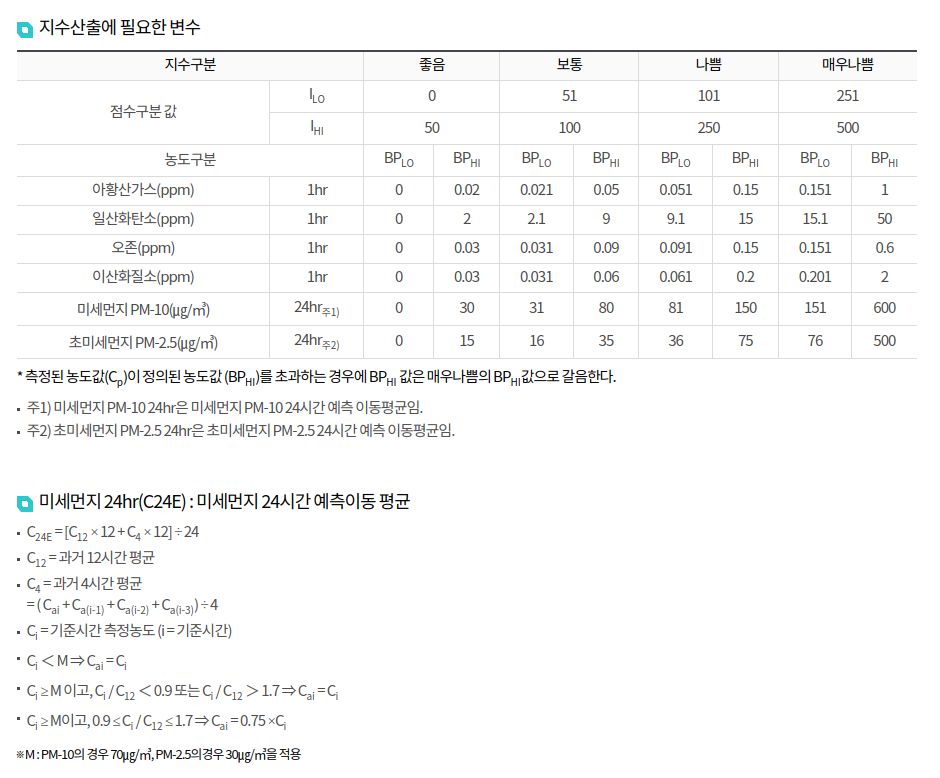
\includegraphics[width=0.85\linewidth]{images/CAI_Korea.png}
		\end{minipage}	
		&
		\begin{minipage}[t]{0.05\textwidth} \scriptsize	

		\end{minipage}
	\end{tabular}
\end{frame}




\begin{frame}[t]{배출량과 성장분야의 비교}
	\begin{tabular}{ll}
		\begin{minipage}[t]{0.475\textwidth}\scriptsize
			\begin{figure}[t]
				\includegraphics[trim=330 50 50 425, clip, 
				page=401, width=\textwidth]{\bookfile}
			\end{figure}
		\end{minipage}	
		&
		\begin{minipage}[t]{0.475\textwidth} \scriptsize	
			\questionset{우리나라 대기오염 물질의 농도가 증가하는 물질과 감소하는 물질은 무엇인가?}
			\solutionset{$\rm{{O}_{3}}$의 농도가 증가하는 경향을 보이고 있다. 이는 자동차의 증가로 광화학 스모그가 증가함을 알 수 있다. $\rm{CO}$ㅡ $\rm{SO}_{2}$는 감소하는 경향을 보이고 있다. 석탄 사용이 줄고 천연가스 등 청정 연료 사용에 의한 결과라고 추측해 볼 수 있다.}
				
		\end{minipage}
	\end{tabular}
\end{frame}



\begin{frame}[t]{중국의 대기 오염 사건(2010년 10월)}
	\begin{tabular}{lll}
		\begin{minipage}[t]{0.32\textwidth}\scriptsize
			\begin{figure}[t]
				\includegraphics[trim=30 40 350 420, clip, 
				page=403, width=\textwidth]{\bookfile}
			\end{figure}
		\end{minipage}	
		&
		\begin{minipage}[t]{0.31\textwidth}\scriptsize
			\begin{figure}[t]
				\includegraphics[trim=330 470 165 110, clip, 
				page=403, width=\textwidth]{\bookfile}
			\end{figure}
		\end{minipage}	
		&
		\begin{minipage}[t]{0.31\textwidth}\scriptsize
			\begin{figure}[t]
				\includegraphics[trim=330 240 165 340, clip, 
				page=403, width=\textwidth]{\bookfile}
			\end{figure}
		\end{minipage}	
	\end{tabular}
	
	중국에서 배출된 대기오염 물질은 편서풍을 타고 우리나라에 영향을 준다.

\end{frame}



\section{대기 오염에 영향을 주는 기상학적 요소}

\begin{frame}[t]{바람의 영향}
	\begin{tabular}{ll}
		\begin{minipage}[t]{0.6\textwidth}\scriptsize
			\begin{figure}[t]
				\includegraphics[trim=50 40 290 540, clip, 
				page=402, width=\textwidth]{\bookfile}
			\end{figure}
		\end{minipage}	
		&
		\begin{minipage}[t]{0.35\textwidth} \scriptsize	
			\begin{itemize}
				\item 풍속이 약하면 풍속이 강할 때보다 대기 오염 현상 발생 가능성 큼
				\item 풍속이 강하면 더 강한 난류(turbulent)가 발생하여 주변 공기와 혼합을 빠르게 시켜서 오염물질을 많이 희석시킴
				\item 대기 오염에 영향을 주는 가장 큰 요인은 대기로 방출되는 오염 물질의 양이지만, 꾸준하게 장기간 배출되더라도 하루하루 대기질의 변동은 매우 크게 나타남.				
			\end{itemize}

		\end{minipage}
	\end{tabular}
\end{frame}



\begin{frame}[t]{혼합층 깊이(mixing depth)}
	\begin{tabular}{ll}
		\begin{minipage}[t]{0.5\textwidth}\scriptsize
			\begin{figure}[t]
				\includegraphics[trim=0 440 350 0, clip, 
				page=404, width=\textwidth]{\bookfile}
			\end{figure}
		\end{minipage}	
		&
		\begin{minipage}[t]{0.45\textwidth} \scriptsize	
			혼합층 깊이(mixing depth): 지표와 대류가 일어나는 높이까지의 연직방향 높이
			\begin{itemize}
				\item 혼합층 깊이가 커질수록 대기질은 개선
				\item 오전보다는 오후에, 겨울보다는 여름에 큼
				\item 대기가 안정하면, 대류가 잘 일어나지 않고 혼합 깊이가 작음
				\item 대기가 불안정하면, 대류가 잘 일어나고 혼합 깊이가 커짐
				\item 기온 역전은 대기가 안정하고 혼합층 깊이가 크게 제한. 
				\item 연직운동이 제한되어 지표 부근에 오염 물질 갇힘
					
			\end{itemize}

		\end{minipage}
	\end{tabular}
\end{frame}



\begin{frame}[t]{대기 안정도의 영향}
	\begin{tabular}{ll}
		\begin{minipage}[t]{0.475\textwidth}\scriptsize
			\begin{figure}[t]
				\includegraphics[trim=350 240 50 380, clip, 
				page=404, width=\textwidth]{\bookfile}
			\end{figure}
		\end{minipage}	
		&
		\begin{minipage}[t]{0.475\textwidth}\scriptsize
			\begin{figure}[t]
				\includegraphics[trim=350 60 50 562, clip, 
				page=404, width=\textwidth]{\bookfile}
			\end{figure}
		\end{minipage}
	\end{tabular}
	
	지표 기온역전: 밤에는 복사 냉각으로 지표부근 기온 역전 발생.
		\begin{itemize} \scriptsize	
		\item 일출 후에는 지표가 가열되므로 역전층이 점차 사라짐
		\item 평탄하지 않은 지역에서는 차가운 공기가 고지대와 경사지로부터 서서히 저지대와 협곡에 흘러 들어 역전이 형성되며, 이러한 역전은 일출 후에도 빨리 소멸되지 않음
			
	\end{itemize}
\end{frame}



\begin{frame}[t]{대기 안정도의 영향}
	\begin{tabular}{ll}
		\begin{minipage}[t]{0.475\textwidth}\scriptsize
			\begin{figure}[t]
				\includegraphics[trim=40 500 350 50, clip, 
				page=405, width=\textwidth]{\bookfile}
			\end{figure}
		\end{minipage}	
		&
		\begin{minipage}[t]{0.475\textwidth} \scriptsize	
			상층 기온역전: 고기압 중심부터 발생하는 침강 공기에 의해 발생
			\begin{itemize}
				\item LA의 대기 오염은 북태평양 고기압의 하강기류로 인한 상층 역전으로 빈번하게 발생
			\end{itemize}
			
			\questionset{대기의 상층에서 발생하는 역전과 접지 역전을 비교하여 설명하시오.}
			\solutionset{접지 역전은 보통 밤동안의 지표의 강한 복사 냉각이나, 따뜻한 공기가 차가운 지표나 해수면에 의해 냉각될 때 나타난다. 반면 상층 역전은 고기압의 중심에서 공기가 침강하거나 전선면에서 따뜻한 공기가 차가운 공기 위로 강제 상승할 때 발생한다.}
		\end{minipage}
	\end{tabular}
\end{frame}



\begin{frame}[t]{}
	\begin{tabular}{ll}
		\begin{minipage}[t]{0.475\textwidth}\scriptsize
			\questionset{대기 오염에 영향을 주는 두 가지 대기 조건을 설명하시오.}
			\solutionset{바람의 강도와 대기의 안정도가 대기 오염에 영향을 미친다. 
				바람이 약하거나 없을 때는 오염 물질을 빨리 이동시키지 못하고, 난류가 약해 고농도의 오염공기를 희석시키지 못해 오랫동안 체류하게 만들어 대기 오염이 심화된다. 
				기온 역전은 연직 방향의 운동을 제한하여 오염 물질이 지표의 좁은 지역에 머물게 함으로써 대기 오염을 심화 시킨다.}

		\end{minipage}	
		&
		\begin{minipage}[t]{0.475\textwidth} \scriptsize	
			
		\end{minipage}
	\end{tabular}
\end{frame}





\section{산성비}

\begin{frame}[t]{산성비}
	\begin{tabular}{ll}
		\begin{minipage}[t]{0.6\textwidth}\scriptsize
			\begin{figure}[t]
				\includegraphics[trim=0 410 200 50, clip, 
				page=406, width=\textwidth]{\bookfile}
			\end{figure}
		\end{minipage}	
		&
		\begin{minipage}[t]{0.35\textwidth} \scriptsize	
			\begin{itemize}
				\item 자연에서는 대기 중의 이산화탄소가 수증기에 녹으면서 약간의 탄산이 생성되어, 일반적인 비의 pH는 $5.6 \sim 6.5$의 분포를 가짐
				\item 자연 상태보다 산성도가 높은 pH가 5.6 미만인 비를 산성비라고 부름			
			\end{itemize}

		\end{minipage}
	\end{tabular}
\end{frame}



\begin{frame}[t]{산성비의 원인}
	\begin{tabular}{ll}
		\begin{minipage}[t]{0.475\textwidth}\scriptsize
			황 산화물(이산화 황, 삼산화 황 등)
			\begin{itemize}
				\item 황을 포함하는 화석연료가 연소할 때 발생하며, 보통은 자동차 연소보다는 공장에서 황산 등을 제조할 때 주로 생김
				\item 물방울에 용해되어 황산을 만들어 산성도를 높임

			\end{itemize}

		\end{minipage}	
		&
		\begin{minipage}[t]{0.475\textwidth} \scriptsize	
			질소 산화물(일산화 질소, 이산화 질소 등)			
			\begin{itemize}
				\item 공기 중 화석연료 등 물질 연소(보통 자동차 연소)시 부산물로 발생
				\item 물방울에 용해되어 질산을 만들어 산성도를 높임
			
			\end{itemize}

		\end{minipage}
	\end{tabular}
\end{frame}



\begin{frame}[t]{우리나라의 산성비}
	\begin{tabular}{ll}
		\begin{minipage}[t]{0.475\textwidth}\scriptsize

			외국과 다른 특징을 보임

			\begin{itemize}
				\item (외국) 초기 강우의 pH가 낮고, 시간이 갈수록 pH가 높아짐
				\item (우리나라) 초기 강우의 pH가 높고, 시간이 갈수록 pH가 낮아지거나 일정하게 유지
						→ 대기 중의 먼지는 강우에 의해 제거되기 쉬운데, 우리나라의 경우 대기 중의 먼지가 많은 편이기 때문에 먼지가 초기 강우 시 흡수되어 빗물을 중화시키기 때문에 초기 pH가 높음.
			   
			\end{itemize}

		\end{minipage}	
		&
		\begin{minipage}[t]{0.475\textwidth} \scriptsize	
			
			우리나라 산성비 특성은 빗물을 중화해 주는 분진 때문에 나타남
			\begin{itemize}
				\item 황사 현상이 있을 때나 대기 중의 분진이 다량 존재할 경우, pH 7 이상인 알칼리성 비가 내리기도 함.
				\item 부유 분진의 관점에서 보면 황사는 문제 현상이나 산성비의 관점에서는 중요한 중화제 공급처이기도 함.
				
			\end{itemize}

		\end{minipage}
	\end{tabular}
\end{frame}



\begin{frame}[t]{산성비의 영향}
	\begin{tabular}{ll}
		\begin{minipage}[t]{0.5\textwidth}\scriptsize
			\begin{figure}[t]
				\includegraphics[trim=330 450 0 50, clip, 
				page=407, width=\textwidth]{\bookfile}
			\end{figure}
		\end{minipage}	
		&
		\begin{minipage}[t]{0.45\textwidth} \scriptsize	
			\questionset{산성비가 환경에 미치는 영향을 기술하시오.}
			\solutionset{인간의 건강: 몸에 해로운 입자를 제거하는 기능을 하는 기관지와 폐 기능 약화

			환경: 호수와 강의 산성도 증가, 어류 서식이 불가능해 짐, 토양의 산성화로 농작물과 산림 생산성 감소

			구조물: 철구조물과 석재 조형물을 파괴}	
		\end{minipage}

	\end{tabular}
\end{frame}



\begin{frame}[t]{산성비에 대한 대책}
	\begin{tabular}{ll}
		\begin{minipage}[t]{0.475\textwidth}\scriptsize
			
			황 산화물, 질소 산화물을 대기 중으로 배출하지 않는 것이 대책의 기본
			\begin{itemize}
				\item 자동차 사용 억제 등 에너지 절약 정책 추진
				\item 청정연료 사용을 권장하며 보급
				\item 발전소나 공장에 탈황, 탈질 설비를 설치
				\item 자동차 배출가스 정화장치 부착
				\item 에너지 효율을 높이기 위한 에너지 사용방식 개선
				\item 산성화된 토양이나 호소를 복원하는 방법으로 토양이나 삼림에 석회를 살포하거나 호소를 중화시키는 방법 등
				
			\end{itemize}
			
		\end{minipage}	
		&
		\begin{minipage}[t]{0.475\textwidth} \scriptsize	
		
		\end{minipage}

	\end{tabular}

\end{frame}
